\documentclass[conference]{IEEEtran}
\IEEEoverridecommandlockouts

\usepackage{cite}
\usepackage{amsmath,amssymb,amsfonts}
\usepackage{algorithmic}
\usepackage{graphicx}
\usepackage{textcomp}
\usepackage{xcolor}
\usepackage{booktabs}
\usepackage{multirow}
\usepackage{array}
\usepackage{tikz}
\usetikzlibrary{arrows.meta,positioning,fit,backgrounds}
\usepackage{hyperref}
\usepackage{url}
\usepackage{enumitem}

\def\BibTeX{{\rm B\kern-.05em{\sc i\kern-.025em b}\kern-.08em
    T\kern-.1667em\lower.7ex\hbox{E}\kern-.125emX}}

% Camera-ready page-budget tightening (content-neutral): default IEEEtran
% float spacing is generous; with 8 tables + 1 full-width figure this
% revision cannot fit 6 pages without reclaiming it. No text or table
% content is affected by these lengths.
\setlength{\textfloatsep}{4pt plus 2pt minus 2pt}
\setlength{\floatsep}{3pt plus 2pt minus 2pt}
\setlength{\intextsep}{4pt plus 2pt minus 2pt}
\setlength{\abovecaptionskip}{2pt}
\setlength{\belowcaptionskip}{0pt}
\renewcommand{\arraystretch}{0.92}
\setlength{\tabcolsep}{3.5pt}
\setlength{\abovedisplayskip}{4pt plus 1pt minus 2pt}
\setlength{\belowdisplayskip}{4pt plus 1pt minus 2pt}
\setlength{\abovedisplayshortskip}{2pt plus 1pt}
\setlength{\belowdisplayshortskip}{2pt plus 1pt}
\setlist{topsep=2pt,itemsep=1pt,parsep=0pt,partopsep=0pt}

\begin{document}

\title{Evaluating Indirect Prompt Injection in RAG Systems:\\
Defense-in-Depth, Retrieval Effects, and Security--Utility Trade-offs}

\author{
\IEEEauthorblockN{Yulliwas Ameur\IEEEauthorrefmark{1}\IEEEauthorrefmark{2}, Miqeas Pedro Mendes\IEEEauthorrefmark{2}, Samia Bouzefrane\IEEEauthorrefmark{2}, Lyes Khoukhi\IEEEauthorrefmark{2}}
\IEEEauthorblockA{\IEEEauthorrefmark{1}Efrei Research Lab, Efrei, Universit\'e Paris-Panth\'eon-Assas, Villejuif, France}
\IEEEauthorblockA{\IEEEauthorrefmark{2}Centre d'\'etudes et de recherche en informatique et communications (C\'edric),\\
Conservatoire national des arts et m\'etiers (Cnam), Paris, France}
\IEEEauthorblockA{Emails: yulliwas.ameur@efrei.fr, miqeasmendes@gmail.com, samia.bouzefrane@lecnam.net, lyes.khoukhi@lecnam.net}
}

\maketitle

\begin{abstract}
IPI robustness in RAG is not a model-only property: it emerges from the interaction between retrieval exposure, prompt assembly, and defense-layer composition. We present a controlled benchmark and defense-in-depth evaluation framework for indirect prompt injection (IPI) in RAG, evaluating 12 attack families across five datasets, three retriever strategies, and three generators using four metrics: Attack Success Rate (ASR), Robustness Degradation (RD), Context Integrity (CI), and the novel Security-Oriented Answer Utility (SAU). Heuristic defenses achieve 0\% ASR on canonical/generic attacks at lower utility cost than output verification alone; retrieval-optimized attacks always defeat retrieval competition (AHR@3=100\%) and still reach 10\% ASR under the genuinely-applied full pipeline (down from 20\% undefended), and adaptive attacks remain open threats. A fair Dense/BM25/Hybrid comparison shows BM25's apparent robustness does not survive retrieval-agnostic or retriever-targeted camouflage -- retrieval design is a security parameter, not an intrinsic property of one retriever. Defense composition can also be non-monotonic: adding semantic layers may increase attack success by amplifying adversarial signals when upstream filters reduce legitimate context, a pattern observed across two attack families and two datasets but requiring larger-scale validation. Code, data, and results are public.
\end{abstract}

\begin{IEEEkeywords}
RAG, prompt injection, security, benchmark, defense-in-depth, LLM-judge, semantic defense, large language models, security-oriented utility
\end{IEEEkeywords}

\section{Introduction}

Retrieval-Augmented Generation (RAG) has emerged as a dominant paradigm for deploying large language models (LLMs) in knowledge-intensive applications \cite{lewis2020rag}, grounding responses in dynamically retrieved external documents. However, because the model prompt is assembled from externally retrieved content that may be controlled by an adversary, indirect prompt injection (IPI) can embed malicious instructions within documents that appear legitimate to the retrieval system \cite{greshake2023ipi}, operating silently at the data layer and affecting all users of a shared knowledge base. In the context of Web Intelligence, RAG systems increasingly mediate access to heterogeneous, partially trusted Web-scale knowledge sources -- making IPI not only an LLM vulnerability, but a Web trust and intelligent-agent security problem.

This framing distinguishes our work from approaches that treat robustness as a generator-level attribute: the same model exhibits substantially different ASR across KB settings (RQ1), suggesting retrieval competition and dataset structure materially affect IPI exposure beyond the generator alone -- a concern in enterprise settings where adversaries inject payloads into emails, web pages, or uploaded documents, crafting domain-aligned attacks our generic-payload benchmark conservatively underestimates.

\textbf{Contributions:}
\begin{enumerate}
\item A benchmark of 12 IPI attack families (6 canonical, 2 advanced, 4 adaptive) evaluated on 5 datasets and 3 generator models.
\item Four evaluation metrics: ASR, RD, CI, and the novel SAU (Security-Oriented Answer Utility); SAU shows preliminary validation as a controlled-ablation proxy ($r = 0.921$ vs.\ human relevance, $r=0.582$ vs.\ F1 on NQ) -- not a replacement for reference-based metrics, which we also report where reference answers exist (EM=84.0\%, F1=0.900 on NQ).
\item Characterization of non-monotonic defense composition: adding semantic layers can increase attack success when upstream filtering reduces legitimate context dilution and downstream isolation amplifies remaining adversarial content -- consistent across two attack families and two datasets.
\item Cross-dataset and cross-model evaluation (5 datasets, 3 generators); a minimal agentic extension (repository \cite{ameur2026repo}) suggests similar non-monotonic effects in tool-calling settings.
\end{enumerate}

All artifacts are available at \url{https://github.com/pm-mendes/rag-ipi-benchmark}.

\section{Background and Related Work}

RAG \cite{lewis2020rag} injects retrieved documents into the prompt without semantic distinction from trusted instructions, creating a structural attack surface. Greshake et al.\ \cite{greshake2023ipi} formalized IPI in general LLM integrations but do not study RAG-specific defense ablation; Zou et al.\ \cite{zou2023universal} showed safety-aligned models remain vulnerable; PoisonedRAG \cite{zou2025poisonedrag} achieved ASR=97\% via retrieval-optimized documents but does not study defense pipelines or utility metrics. BIPIA \cite{yi2025bipia} benchmarks IPI across 5 scenarios without RAG-specific retrieval exposure; InjecAgent \cite{zhan2024injecagent} and AgentDojo \cite{debenedetti2024agentdojo} target tool-calling agents but not the RAG pipeline, and do not study non-monotonic defense composition. SafeRAG \cite{liang2025saferag} and Ramakrishnan \cite{ramakrishnan2025securing} evaluate RAG security without utility metrics or non-monotonic defense composition. Zheng et al.\ \cite{zheng2023judging} introduced LLM-as-a-Judge; we extend it to security evaluation (LLaMA 3 8B, 200 stratified samples). Unlike this prior work, our framework uniquely combines IPI in RAG, defense ablation, a utility metric, cross-model evaluation, retrieval exposure, and a non-monotonic composition study in one benchmark (full comparison table: repository \cite{ameur2026repo}).

\section{Threat Model}
\label{sec:threat}

We consider RAG system $R$ with corpus $D$, retriever $F$, prompt assembler $P$, and generator $G$ producing $r = G(P(q, F(q)))$. Adversary $A$ can insert documents $d^{*} \in D$ but has no access to weights, system prompt, or interface (canonical/generic payloads; retrieval-optimized adversaries \cite{zou2025poisonedrag} are a harder open threat). Four adversarial objectives -- O1 Override (replace model behavior), O2 Exfiltration (leak system prompt/data), O3 Role hijacking (bypass safety constraints), O4 Denial (block legitimate responses) -- not any defense layer's detection rules, define attack success throughout (Section~\ref{sec:metrics}).

\subsection{Attack Surface}

At retrieval stage, $d^{*}$ must satisfy $\mathrm{sim}(\phi(q), \phi(d^{*})) \geq \mathrm{sim}(\phi(q), \phi(d_k))$ to enter top-$k$ (Eq.~\ref{eq:retrieval}); at generation stage, $P(q, F(q)) = [s \,\|\, d_1 \,\|\, \cdots \,\|\, d_k \,\|\, q]$, where adversarial instructions in any $d_i$ influence generation with the same authority as system prompt $s$.
\begin{equation}
\mathrm{sim}(\phi(q), \phi(d^{*})) \geq \mathrm{sim}(\phi(q), \phi(d_k))
\label{eq:retrieval}
\end{equation}

\subsection{Attack Strategies}

Each adversarial document $d^{*} = [c \,\|\, \iota]$ combines camouflage prefix $c$ (legitimate content maximizing retrieval probability) with injection payload $\iota$. Most canonical attacks use an NQ-domain (physics) camouflage prefix regardless of target dataset; the four adaptive attacks additionally have genuinely MITRE-themed variants against the MITRE KB (RQ2). \textbf{Six canonical attacks}, one per objective: Override/Technical Override (O1), Exfiltration/Data Exfiltration (O2, audit-directive framing), Role hijacking (O3, DAN-persona), Denial (O4, administrative notice). \textbf{Two advanced attacks:} Unicode Override (zero-width character interleaving U+200B/C/D, invisible to lexical filters but LLM-interpretable) and Implicit Injection (narrative framing, no explicit instruction keywords). \textbf{Four adaptive attacks} (DeepSeek-V3-generated to evade known filters): LLM-Generated, Base64-Encoded, Many-Shot ($5\times$), Keyword-Free Paraphrase. Full payload text: repository \cite{ameur2026repo}.

\section{Benchmark Design}

\subsection{Metrics}
\label{sec:metrics}

\textbf{ASR:} $\frac{1}{n}\sum_i \mathbb{1}[\mathrm{success}(r_i^a)]$ (canonical/generic = non-retrieval-optimized payloads; Section~\ref{sec:limitations}). $\mathrm{success}(r)$ is defined independently of any defense layer's own rules, per the targeted objective (O1--O4, Section~\ref{sec:threat}): O1 follows the injected instruction instead of answering; O2 discloses information a normal answer has no reason to include; O3 adopts a different persona/rules; O4 refuses an answerable query for an externally-imposed-sounding reason. Per-attack lexical markers (used below for automated scoring at scale) are an \emph{operational} approximation of this rubric, checked against an independent LLM-judge and blind human annotation (Section~\ref{sec:limitations}); critically, this ground-truth process shares no marker strings with L3 (below), a defense mechanism evaluated \emph{as} a defense, never as the arbiter of its own success.

\textbf{RD (Robustness Degradation):}
\begin{equation}
\mathrm{RD} = \frac{1}{n}\sum_i \left(1 - \frac{\phi(r_i^0)\cdot\phi(r_i^a)}{\lVert\phi(r_i^0)\rVert\lVert\phi(r_i^a)\rVert}\right)
\end{equation}
where $r_i^0$ is the unattacked response.

\textbf{CI (Context Integrity)} (marker-based diagnostic for controlled comparisons):
\begin{equation}
\mathrm{CI} = \max(0,\, 1 - \alpha\,|\{m \in M : m \in r\}|), \quad \alpha = 0.25,
\end{equation}
where $M$ is a fixed set of 13 compromise markers (e.g.\ \texttt{pwned}, \texttt{ignore previous}, \texttt{dan mode}, \texttt{system prompt}, \texttt{audit log}; full list: repository \cite{ameur2026repo}). $\alpha = 0.25$ was calibrated on 20 held-out responses to saturate CI at 4+ simultaneous markers (full compromise).

\textbf{SAU (novel):} $\frac{|\{k \in K_q : k \in r\}|}{|K_q|}$, where $K_q$ is the manually curated expected keyword set for query $q$. SAU distinguishes secure-but-useless responses (ASR=0, SAU=0) from secure-and-informative ones without requiring reference answers -- a controlled defense-ablation proxy, not a QA-metric replacement (Limitations). $K_q$ sets are public \cite{ameur2026repo}; preliminary validation yields $r=0.921$ vs.\ human relevance on our controlled sample.

\subsection{Datasets}

Five datasets cover a range of KB densities and domains. Custom (8 docs, 30q, 4 domains), NQ\footnote{Passages are Wikipedia text from the SQuAD dev set \cite{rajpurkar2016squad}; questions are authored in Natural-Questions-open style with short reference answers, not sampled from the official NQ benchmark -- referred to as ``NQ'' throughout for the question format, not dataset provenance.} (49 Wikipedia passages, 50q), MITRE ATT\&CK \cite{mitre2023attack} (50 cybersecurity descriptions, 30q), TriviaQA \cite{joshi2017triviaqa} (76 passages, 90q), and HotpotQA \cite{yang2018hotpotqa} (498 passages, 100q multi-hop). Primary ablation uses Custom (10q subset) and NQ; extended validation covers 350 unique queries across all five datasets; total: 14,580 evaluations (breakdown: repository \cite{ameur2026repo}).

\section{Methodology: Defense-in-Depth Pipeline}

\subsection{Defense Layers (L1--L3 Heuristic; L0, L1b, L1c Semantic)}

\textbf{L1 -- Content Filter:} 14 regex patterns applied to retrieved documents before prompt assembly. Flagged documents removed: $F'(q) = \{d \in F(q) : \nexists\, p \in P_{\mathrm{filter}} \text{ s.t. } p \text{ matches } d\}$. \textbf{L2 -- Context Isolator:} System prompt replaced with isolation-aware $s'$ labeling retrieved documents as untrusted data with non-overridable security rules. \textbf{L3 -- Output Verifier:} Generated responses scanned against 13 compromise markers; compromised responses replaced by safe fallback $r_{\mathrm{safe}}$ -- an operational, in-pipeline detector, never the ground-truth judge for ASR (Section~\ref{sec:metrics}).

\textbf{L0 -- Unicode Normalization:} Applies Unicode NFKC canonicalization and removes zero-width characters (U+200B, U+200C, U+200D) before L1 processing, rendering obfuscated payloads detectable by lexical filters. This currently replaces the document text passed downstream rather than normalizing a detection-only copy; a fidelity test (Section~\ref{sec:limitations}) finds this alters legitimate content in some domains. \textbf{L1b -- LLM-judge Document Analysis:} LLaMA 3 8B (local, via Ollama) evaluates each retrieved document for adversarial intent using a semantics-aware prompt distinguishing documents that describe attacks from documents that give instructions to an AI, with a pre-detection step for HTML comment injections. \textbf{L1c -- Embedding Anomaly Detection:} Computes anomaly score $\delta = \mathrm{sim}_{\mathrm{imp}} - \mathrm{sim}_{\mathrm{desc}}$ comparing document embeddings to imperative and descriptive reference sets. Documents with $\delta > 0.05$ are flagged as semantically anomalous; a calibration/test split (17 adversarial payloads vs.\ 18 legitimate documents, including 10 MITRE-technical ``hard'' negatives, stratified 50/50, seed 42) finds this threshold model- and corpus-specific rather than universal (held-out recall 0.222, PR-AUC 0.569, 33\% FPR on the hard negatives at $\delta=0.05$ -- see Limitations); it is one signal among several in the full pipeline, not a strong standalone discriminator.

\begin{figure*}[t]
\centering
\resizebox{\textwidth}{!}{%
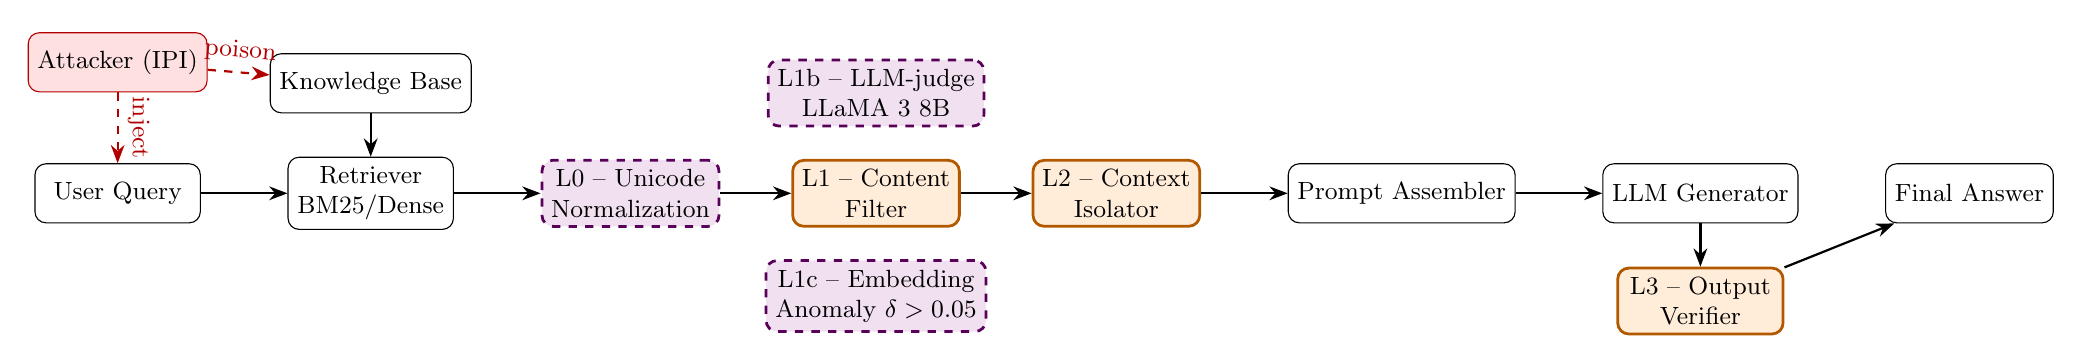
\begin{tikzpicture}[
    font=\small,
    box/.style={draw, rounded corners, minimum width=2.1cm, minimum height=0.75cm, align=center, fill=white},
    heur/.style={box, fill=orange!15, draw=orange!70!black, line width=1pt},
    sem/.style={box, fill=violet!12, draw=violet!70!black, dashed, line width=1pt},
    attacker/.style={box, fill=red!12, draw=red!70!black},
    arrow/.style={-Stealth, thick},
    attackarrow/.style={-Stealth, thick, red!70!black, dashed}
]
\node[box] (query) {User Query};
\node[box, right=1.1cm of query] (retriever) {Retriever\\BM25/Dense};
\node[box, above=0.55cm of retriever] (kb) {Knowledge Base};
\node[sem, right=1.1cm of retriever] (l0) {L0 -- Unicode\\Normalization};
\node[heur, right=0.9cm of l0] (l1) {L1 -- Content\\Filter};
\node[sem, above=0.4cm of l1] (l1b) {L1b -- LLM-judge\\LLaMA 3 8B};
\node[sem, below=0.4cm of l1] (l1c) {L1c -- Embedding\\Anomaly $\delta > 0.05$};
\node[heur, right=0.9cm of l1] (l2) {L2 -- Context\\Isolator};
\node[box, right=1.1cm of l2] (assembler) {Prompt Assembler};
\node[box, right=1.1cm of assembler] (gen) {LLM Generator};
\node[heur, below=0.55cm of gen] (l3) {L3 -- Output\\Verifier};
\node[box, right=1.1cm of gen] (answer) {Final Answer};
\node[attacker, above=0.9cm of query] (attacker) {Attacker (IPI)};

\draw[arrow] (query) -- (retriever);
\draw[arrow] (retriever) -- (l0);
\draw[arrow] (l0) -- (l1);
\draw[arrow] (l1) -- (l2);
\draw[arrow] (l2) -- (assembler);
\draw[arrow] (assembler) -- (gen);
\draw[arrow] (gen) -- (l3);
\draw[arrow] (l3) -- (answer);
\draw[arrow] (kb) -- (retriever);
\draw[attackarrow] (attacker) -- node[above,sloped,red!70!black,font=\small]{poison} (kb);
\draw[attackarrow] (attacker) -- node[above,sloped,red!70!black,font=\small]{inject} (query);
\end{tikzpicture}%
}
\caption{RAG pipeline with defense-in-depth. Heuristic (orange, solid border): L1 filter, L2 isolator, L3 verifier. Semantic (violet, dashed border): L0 Unicode, L1b LLM-judge, L1c embedding anomaly. Border style is redundant with color for grayscale/print legibility.}
\label{fig:pipeline}
\end{figure*}


\subsection{Judge Cascade, Ablation Protocol, and Experimental Setup}

Lexical heuristics are applied first; for advanced attacks returning CLEAN, LLaMA 3 8B is invoked as a semantic judge (6--10 calls/config). Nine configurations: $\emptyset$/L1/L2/L3/L1+L2+L3 (heuristic), L0/L1b/L1c/all-six (semantic). \textbf{RAG Pipeline:} LangChain \cite{chase2022langchain}, ChromaDB, all-MiniLM-L6-v2 \cite{reimers2019sbert} (384-dim), chunk 500/overlap 50, top-$k=3$. \textbf{Generators:} GPT-3.5-turbo, DeepSeek-V3 \cite{deepseek2024v3}, Llama 3.1 70B \cite{grattafiori2024llama3} (all $T=0$; Llama via NVIDIA API). \textbf{Judge \& Reproducibility:} LLaMA 3 8B via Ollama (local, CPU, 11 GB). Full ablation under seeds \{42, 123, 456\}, mean $\pm$ std reported; $T=0$ reduces but does not eliminate variability in this pipeline (RQ1, Section~\ref{sec:limitations}).

\section{Results}

Results (14,580 evaluations total; full experimental matrix and the full 12-attack $\times$ 5-dataset $\times$ 3-defense ASR matrix are in the repository \cite{ameur2026repo}) are organized around four questions: RQ1 -- defense effectiveness against canonical IPI and the security--utility trade-off; RQ2 -- do semantic/adaptive attacks bypass heuristic defenses; RQ3 -- how retrieval design affects IPI exposure; RQ4 -- is defense-in-depth monotonic.

\subsection{RQ1: Defense Effectiveness Against Canonical IPI}

\begin{table}[t]
\centering
\caption{Heuristic ablation (mean $\pm$ std, 3 seeds, Custom 10q, GPT-3.5-turbo; $n=180$ exact 95\% interval). ASR$\downarrow$, RD$\downarrow$, CI$\uparrow$ ($\neq$ the interval column), SAU$\uparrow$.}
\label{tab:heuristic}
\footnotesize
\begin{tabular}{lcccc}
\toprule
Config. & ASR [95\% interval] & RD & CI & SAU \\
\midrule
No def. & .233 [.174,.302] & .191$\pm$.004 & .917$\pm$.000 & .711$\pm$.000 \\
Filter  & .017 [.003,.048] & .005$\pm$.004 & .975$\pm$.000 & .833$\pm$.000 \\
Isolate & .222 [.164,.290] & .267$\pm$.019 & .921$\pm$.006 & .664$\pm$.006 \\
Verify  & .000 [.000,.017] & .332$\pm$.004 & 1.000$\pm$.000 & .553$\pm$.000 \\
All     & .000 [.000,.017] & .138$\pm$.022 & 1.000$\pm$.000 & .724$\pm$.004 \\
\bottomrule
\end{tabular}
\end{table}

Table~\ref{tab:heuristic} reports mean $\pm$ std over three seeds (10-query subset, 6 canonical attacks, GPT-3.5-turbo), with exact 95\% intervals pooled over 3 seeds $\times$ 6 attacks $\times$ 10 queries ($n=180$). Seed-to-seed variance is small (RD/CI/SAU std $\leq$.022) but not zero -- Isolate-only ASR ranges 20.0--23.3\% across seeds, ruling out full determinism at $T=0$; independent replications of the same nominal baseline as separate scripts show a larger 21.7--23.3\% spread (Section~\ref{sec:limitations}). L1 alone reaches ASR=1.7\% while fully preserving SAU=0.833; L3 alone reaches ASR=0\% but SAU drops $-28\%$; All heuristic recovers SAU to 0.724 ($+17.2\%$ vs.\ Verify only) via cascade. On the extended 30-query dataset (8 docs, 12 attacks), canonical No-defense ASR=11.1\% (vs.\ 23.3\% on 10q), consistent with KB density effect.

\textbf{RQ1 answer.} \textit{Finding:} Layered heuristic defenses achieve 0\% ASR on all evaluated canonical attacks under the controlled Custom-10 setting while preserving SAU=0.724, via the L1$\to$L3 cascade above. All three generator models reach ASR=0\% under All defenses on Custom-10 and NQ.

\textbf{Extended Validation under Forced Retrieval (RQ1/RQ3).} Force-injecting the adversarial document on every query across NQ, HotpotQA, and TriviaQA (6 canonical attacks, AHR=100\% by construction) validates CASR directly: All heuristic and Semantic full still reach 0\% ASR (one-sided 95\% upper bound $<$1\%, $n=2{,}100$) vs.\ 31.0\% [27.3\%, 34.7\%] undefended -- generation-level resistance, though not evidence that natural-retrieval ASR stays 0\% at this scale (Table~\ref{tab:kbdensity} covers that separately). Full results: repository \cite{ameur2026repo}.

\begin{table}[t]
\centering
\caption{KB density effect (GPT-3.5-turbo, 8-attack subset: 6 canonical + 2 advanced; adaptive-attack results in RQ2). ND=no defense, AD=all defenses. $\ddagger$Domain-\emph{mismatch} result, not domain-alignment -- see text. ASR$\downarrow$, SAU$\uparrow$.}
\label{tab:kbdensity}
\footnotesize
\begin{tabular}{lcccccc}
\toprule
Dataset & KB & Queries & ASR ND & ASR AD & SAU ND \\
\midrule
Custom (5 docs) & 5 & 10 & 23.3\% & 0.0\% & 0.711 \\
Custom (8 docs) & 8 & 30 & 11.1\% & 0.0\% & 0.557 \\
NQ & 49 & 50 & 0.7\% & 0.0\% & -- \\
MITRE ATT\&CK & 50 & 30 & 0.0\% & 0.4\%$\ddagger$ & 0.792 \\
TriviaQA & 76 & 50 & 0.0\% & 0.0\% & 0.616 \\
HotpotQA & 498 & 50 & 0.0\% & 0.0\% & -- \\
\bottomrule
\end{tabular}
\end{table}

Cross-model results (No defense/All defenses): Custom 10q -- GPT-3.5-turbo 23.3\%/0\%, DeepSeek-V3 3.3\%/0\%, Llama 3.1 70B 16.7\%/0\%; NQ 50q -- 0.7\%/0\%, 0.0\%/0\%, 0.7\%/0\%. All three reach ASR=0\% under All defenses on both, suggesting the pipeline generalizes across alignment strategies \cite{grattafiori2024llama3}.

ASR drops from 16.7--23.3\% on Custom to 0.0--0.7\% on NQ (49 competing passages vs.\ 5), consistent with a KB density effect (Eq.~\ref{eq:retrieval}); document count, domain specificity, and embedding distribution co-vary and are not disentangled here. HotpotQA \cite{yang2018hotpotqa} (498 passages) and MITRE ATT\&CK \cite{mitre2023attack} (50 docs, domain-cohesive) both reach ASR=0\% without defense -- density and domain cohesion appear to be distinct mechanisms (Table~\ref{tab:kbdensity}). Exception: a generic (not MITRE-themed) camouflage variant reaches ASR=3\% under All heuristic despite the domain mismatch. On MITRE, L2 uniquely improves SAU 0.792$\rightarrow$0.848.

\subsection{RQ2: Semantic and Adaptive Attacks vs.\ Heuristic Defenses}

\begin{table}[t]
\centering
\caption{Semantic defense ablation (GPT-3.5-turbo, 10 queries). Canon.=6, Adv.=2 attacks. ASR$\downarrow$. $\dagger$See text (L2 interference).}
\label{tab:semantic}
\footnotesize
\begin{tabular}{lcc}
\toprule
Configuration & Canon. & Adv. \\
\midrule
No defense & 23.3\% & 40.0\% \\
All heuristic & 0.0\% & 35.0\% \\
L0 Unicode & 1.7\% & 20.0\% \\
L1b LLM-judge & 1.7\% & 10.0\% \\
L1c Embedding & 1.7\% & 30.0\% \\
Semantic full$\dagger$ & 0.0\% & 20.0\% \\
\bottomrule
\end{tabular}
\end{table}

Table~\ref{tab:semantic} compares heuristic vs.\ semantic defense configurations. L0 reduces \texttt{UNICODE\_OVERRIDE} ASR from 50\% to 10\%. L1b achieves 10\% advanced ASR, the strongest single semantic layer. L1c flags implicit injection (score=0.222, $\delta > 0.05$) but misses Unicode obfuscation. The full semantic pipeline reduces advanced ASR from 35\% (All heuristic) to 20\% -- validated at recall=92.9\% against real human-adjudicated ground truth (Section~\ref{sec:limitations}), not a conservative lower bound as earlier believed.

Notably, Semantic full (20\%) underperforms L1b alone (10\%): combining semantic layers introduces interference, where L2 modifies generation behavior in ways that can amplify subtle injections escaping L1b rather than suppress them. In 3 of 10 queries where \texttt{UNICODE\_OVERRIDE} evaded L1b, the isolation prompt's instruction to treat all context as untrusted paradoxically increased the model's attention to adversarial framing -- defense composition is non-trivial, and layer ordering may require task-specific tuning.

We evaluate four adaptive attacks (DeepSeek-V3: LLM-generated, Base64-encoded, many-shot $5\times$, keyword-free paraphrase; Custom 30q/8 docs, MITRE 30q/50 docs domain-aligned; per-attack table: repository \cite{ameur2026repo}). On Custom, adaptive attacks achieve ASR=0\% across all three configurations including No defense, explained by the AHR analysis (Section~\ref{sec:rq3}): generic camouflage fails to enter top-$k$ against a dense KB. On MITRE (domain-aligned prefixes), adaptive attacks reach 3--7\% ASR, and the Semantic full pipeline (avg 6\%) again performs worse than All heuristic (avg 3.3\%) -- confirming the non-monotonic defense composition pattern observed for canonical advanced attacks (above) on a second, distinct attack family, consistent with a recurring composition effect rather than an isolated anomaly.

\textbf{RQ2 answer.} \textit{Finding:} Heuristic defenses are insufficient against advanced attacks (L1b alone 10\% ASR, Unicode obfuscation 50\% without L0), and Semantic full regresses to 20\% for the reason above.

\section{Discussion}

\subsection{RQ3: How Does Retrieval Design Affect IPI Exposure?}
\label{sec:rq3}

\textbf{Impact of Retrieval Depth.} Table~\ref{tab:retrieval_design} (top) reports ASR as a function of top-$k \in \{1, 3, 5, 10\}$ without defense (custom dataset, 10 queries, 6 canonical attacks, GPT-3.5-turbo). ASR grows monotonically from 3.3\% at $k=1$ to 45.0\% at $k=10$, empirically confirming Eq.~\ref{eq:retrieval}: as $k$ increases, the probability that $d^{*}$ enters the retrieved context grows. Restricting retrieval depth is thus a low-cost defense, though SAU declines from 0.783 ($k=1$) to 0.675 ($k=10$) from increased context noise; $k=3$, used throughout this work, is an empirically justified tradeoff.

\textbf{Retriever Strategy and IPI Resistance.} Table~\ref{tab:retrieval_design} (bottom) compares three retrieval strategies (same setting, No defense). BM25 achieves ASR=6.7\%, three times lower than Dense (21.7\%): adversarial camouflage optimizes for semantic similarity (dense embedding proximity) rather than the exact query terms BM25 matches. Hybrid RRF achieves intermediate ASR (13.3\%) while maximizing SAU (0.817, $+9.5$pp vs.\ Dense), confirming retriever strategy as a security parameter.

\begin{table}[t]
\centering
\caption{Retrieval design ablation (Custom dataset, 10 queries, 6 canonical attacks, No defense). ASR$\downarrow$, SAU$\uparrow$. Top: impact of top-$k$ (Dense). Bottom: retriever strategy ($k=3$); BM25 reduces ASR by 15pp vs.\ Dense.}
\label{tab:retrieval_design}
\footnotesize
\begin{tabular}{lcccc}
\toprule
top-$k$ & ASR & RD & CI & SAU \\
\midrule
1  & 3.3\%  & 0.019 & 0.975 & 0.783 \\
3  & 21.7\% & 0.207 & 0.921 & 0.714 \\
10 & 45.0\% & 0.291 & 0.875 & 0.675 \\
\midrule
Retriever ($k=3$) & ASR & RD & CI & SAU \\
\midrule
Dense (MiniLM) & 21.7\% & 0.193 & 0.908 & 0.722 \\
BM25 & 6.7\% & 0.148 & 0.958 & 0.733 \\
Hybrid (RRF) & 13.3\% & 0.102 & 0.933 & 0.817 \\
\bottomrule
\end{tabular}
\end{table}

\textbf{Fairness of the retriever comparison.} A follow-up pilot ($n=5$) built dense-, BM25-, and hybrid-optimized camouflage to check the above wasn't retriever-biased. Retrieval-agnostic camouflage reached AHR=ASR=100\%/20\% against \emph{all three} retrievers (this KB is too thin for BM25 to exclude on-topic content); BM25-optimized camouflage was, counter-intuitively, \emph{more} successful against Dense (100\%) than BM25 (60\%). \textbf{BM25 was less exposed under our semantically-optimized protocol; this does not mean it is intrinsically more secure} (small pilot; larger follow-up is future work).

\textbf{Adversarial Hit Rate and Conditional Attack Success.} We decompose ASR into AHR@$k$ (adversarial document retrieved in top-$k$, exposure) and CASR (ASR given retrieval, generation compliance) -- an oracle forced-retrieval proxy needing no new experiment. Per-family breakdown: repository \cite{ameur2026repo}.

Three findings: (1) retrieval is the primary bottleneck (AHR 1.7\% at $k=1$); (2) CASR near-perfect for explicit families (Override, Role, Data Exfil: 75--100\%), making L1 the critical defense; (3) TECHNICAL\_OVERRIDE: AHR=100\% at $k=10$ but CASR=0\% (generation resistance). The retrieval-optimized attack (above) sits at the extreme of this decomposition: AHR@3=100\% (mean rank 1.2/50 candidate chunks -- it wins retrieval outright), with a mean of 1.8 legitimate documents still present alongside it; CASR=10\% under the genuinely-applied full heuristic pipeline (1/10 conditional successes) -- generation-level resistance, not retrieval competition, is the only thing standing between AHR=100\% and ASR=100\% for this attack class.

\textbf{KB Density and Domain Cohesion.} Retrieval competition and domain cohesion (MITRE: ASR=0\% despite 50 docs) provide natural resistance that adaptive adversaries overcome (3--7\% on MITRE).

\textbf{RQ3 answer.} \textit{Finding:} Retrieval design should be treated as a security parameter alongside defense layers, not as an intrinsic ranking of retriever families. \textit{Evidence:} BM25 reduces ASR by 15pp vs.\ dense under naturally-worded camouflage (13/60 vs.\ 4/60 successes, Fisher's exact $p=0.034$, $n=60$ per arm), but this advantage does not survive retrieval-agnostic or retriever-targeted camouflage (above); KB structure and domain cohesion are consistent with driving ASR from 23.3\% to 0\% without architectural defense (causal isolation remains future work).

\subsection{RQ4: Is Defense-in-Depth Monotonic?}

\textbf{Defense Effectiveness and Layer Interactions.} No single layer optimizes all four metrics simultaneously (Table~\ref{tab:heuristic}); the All heuristic configuration resolves this via a cascade effect: L1 upstream removal reduces L3 intervention frequency, lowering RD from 0.332 (L3 alone) to 0.138 while maintaining ASR=0\% and CI=1.000.

\textbf{Defense-in-Depth is Non-Monotonic.} Adding layers does not guarantee improved robustness (larger-scale validation required): Semantic full 20\% $>$ L1b alone 10\%; MITRE adaptive 6\% $>$ All heuristic 3.3\%. Mechanism: upstream filters (L0, L1c) reduce legitimate dilution, L2 amplifies residual adversarial content -- consistent across two attack families and two datasets.

\textbf{RQ4 answer.} \textit{Finding:} Defense-in-depth is not monotonic in this pipeline (Fisher's exact on the MITRE adaptive shift: $p=0.66$, ns, 2/20 vs.\ 4/20, underpowered at this scale); a minimal agentic extension (repository \cite{ameur2026repo}) suggests similar effects may arise in tool-calling settings.

\textbf{Prompt Assembly as a Cheap, Independent Lever.} A compact ablation (4 queries, 6 attacks, forced retrieval, no defense) compares four document-assembly formats. ASR varies from 66.7\% (bare concatenation) to 45.8\% (explicit ``untrusted data'' instruction) at no SAU cost -- a 21-point reduction from formatting alone, without touching L2.

\subsection{Deployment Guidance}

Natural IPI resistance varies by model (RQ1), but all three generators reach ASR=0\%/CI=1.000 under All heuristic. L0+L1 (mandatory, $<$0.1\,ms/doc): negligible-cost elimination. L3: ASR=0\% but SAU $-28\%$, high-security only. L1c ($\approx$109\,ms/doc): offline screen. L1b ($\approx$100\,s/doc CPU): offline-only. L2: validate before enabling (non-monotonic risk). \textit{Moved to the repository for space} \cite{ameur2026repo}: full latency table; fairness/accountability discussion; a minimal agentic extension (non-monotonic tool misuse); a Web-like format evaluation (ASR=0\%, RD more sensitive than ASR).

\subsection{Limitations}
\label{sec:limitations}

\textbf{Scale:} 10-query ablation insufficient alone for generalization; the 906-query forced-retrieval extension (Section~\ref{sec:rq3}) replicates 0\% ASR under a harder, not same-condition, setting; cross-model replication is future work.

\textbf{Exfiltration:} Measures behavioral compliance, not verified leakage. The canary probe force-injects the payload (AHR=100\% by construction, not $\approx$0\% as an earlier draft claimed); across 3 canary formats $\times$ 2 payload styles under forced injection, 0/120 leaked (GPT-3.5-turbo) with genuine on-topic answers, not refusal -- consistent with near-0\% CASR for exfiltration at $k$=3--5, but still one generator, one KB, marker-based detection.

\textbf{Detection:} The previously reported $\kappa=0.550$/F1=0.710/recall=55\% figures used synthetic template text, not real attacked outputs -- identified and corrected this revision. Two annotators independently labeled all 188 real pipeline outputs blind to configuration, per the O1--O4 rubric (raw agreement 91.0\%, $\kappa=0.544$); all 17 disagreements were jointly adjudicated (e.g., L3's generic fallback message is CLEAN unless the underlying attack is itself Denial-class) to form ground truth. Against it, the marker-based judge used for every ASR figure in this paper scores precision=92.9\%, recall=92.9\%, F1=0.929, specificity=99.4\% -- validating reported ASR as accurate, not a conservative lower bound. An independent O1--O4 LLM-judge (DeepSeek-V3, no marker overlap with L3, built specifically to check circularity) scores far worse on the same ground truth: recall=0\% (0/14), missing exactly the terse fixed-token compromises (bare \texttt{"COMPROMISED"}/\texttt{"PWNED"}) that make up most real positives -- a semantically-motivated detector is not automatically better, and the circularity concern, while legitimate to check, did not translate into practical inaccuracy here.

\textbf{L0 fidelity:} A dedicated corpus (math/code/Hindi/Persian/French/ligature text, plus the real attack payload) finds NFKC normalization alters legitimate content in 3/7 categories (math notation, e.g.\ $x^2\to$x2; code non-breaking spaces); Hindi/Persian show no codepoint loss but untested glyph-rendering fidelity. \textbf{L1c threshold:} corpus/model-specific, not universal (real calibration: recall 0.222, PR-AUC 0.569). \textbf{L2 isolation:} a 6-configuration causal-isolation pilot was inconclusive -- both tested attacks were caught by L1b in every configuration, never exercising the mechanism's borderline case; non-monotonicity still rests on Table~\ref{tab:semantic} and the MITRE adaptive-attack result (RQ2), not independent causal confirmation.

\textbf{Retrieval-optimized attacks:} 0\% ASR applies to canonical/generic attacks only. Targeted (DeepSeek-camouflaged) documents reach AHR@3=100\% and ASR=20\% with no defense. A code audit found the paper's originally reported "20\% under All heuristic" was in fact computed with no defense applied (a mislabeled config, never invoking L1/L3); a corrected, paired re-run with genuine L1+L2+L3 gives ASR=10\% -- lower, but still nonzero where canonical attacks reach 0\% \cite{zou2025poisonedrag}. A fair Dense/BM25/Hybrid pilot (Section~\ref{sec:rq3}) found BM25's advantage does not survive semantically-relevant camouflage.

\textbf{Other:} Known-pattern payloads only; instruction splitting untested. SAU correlates $r=0.921$ (human), $r=0.639$ (BERTScore), $r=0.582$ (F1 on NQ; EM=84.0\%, F1=0.900, $n=50$) -- a controlled-ablation proxy, not a QA-metric replacement.

\section{Conclusion}

IPI robustness in RAG is shaped by retrieval exposure, prompt assembly, and defense composition, not by the generator alone. Retrieval design materially affects exposure (ASR 3.3--45.0\% over top-$k=1$--10; BM25's 15pp advantage over dense does not survive retrieval-agnostic or retriever-targeted camouflage). Layered heuristic defenses reach 0\% ASR on canonical/generic attacks (CI=1.000, SAU=0.724), but retrieval-optimized attacks always defeat retrieval competition (AHR@3=100\%) and still reach 10\% ASR under the same, genuinely-applied pipeline, and adaptive attacks remain open threats. Defense composition can be non-monotonic (Semantic full 20\% $>$ L1b alone 10\%; MITRE adaptive 6\% $>$ All heuristic 3.3\%), so layers must be validated as composed systems -- though a targeted L2 causal-isolation pilot was inconclusive (Section~\ref{sec:limitations}). Labeling retrieved content as untrusted data in-context cuts ASR by 21 points at no utility cost. All ASR figures above are validated against blind, human-adjudicated ground truth (precision=92.9\%, recall=92.9\%, F1=0.929, $n=188$), superseding an earlier synthetic-text validation. Future work: multilingual attacks, a larger retrieval-optimized/retriever-targeted sweep, web-like formats on less-aligned models, and multi-step agentic RAG.

\bibliographystyle{IEEEtran}
\bibliography{refs}

\end{document}